\chapter{Literature Review}
\label{chap:lr}

The structure of the literature review in this chapter is designed to offer an in-depth and complete insight into the concept of model distillation, particularly about the research question at hand. This review aims to elucidate the various facets of model distillation, including its theoretical foundations, practical applications, and relevance to the specific research question being addressed.

\section{Search Process}

Google Scholar was the primary digital platform for sourcing scholarly articles relevant to Knowledge Distillation techniques applied to LLMs. The search was conducted using a predefined set of keywords: \{Distillation, Large Language Model, Classification, Natural Language Processing\}. Furthermore, I scrutinized some references from the acquired articles to deepen my understanding of the subject matter. For a study to be included in this review, it needed to either detail a method of LLM distillation or provide sufficient background information to contextualize the research findings. I also set exclusion criteria; studies were disregarded if they lacked verifiable credibility, as indicated by insufficient citations, absence from prominent conferences, or non-publication in well-regarded scientific journals. Consequently, the majority of the selected studies were sourced from arXiv, where authors and institutes post electronic preprints and post-prints, which are moderated before but not peer-reviewed, and papers from the ACL and NeurIPS conferences, both of which are high-prestige venues with rigorous peer review processes.

\section{Knowledge distillation}

One of the paradigms for deriving a more compact model from a larger one or transferring the knowledge to another model is known as ``knowledge distillation.'' During this process, knowledge from a larger model (often called the teacher model) is transferred to a smaller model (student model). The fundamental premise behind this is that the teacher model has captured a deep understanding of the data, which can be imparted to a student model, ensuring that the smaller model performs at a level comparable to its bigger counterpart without consuming the same computational resources. This methodology initially became widespread for classification tasks within the realm of computer vision and has been effectively utilized across various fields, including LLMs.

\begin{figure}[hbt]
    \centering
    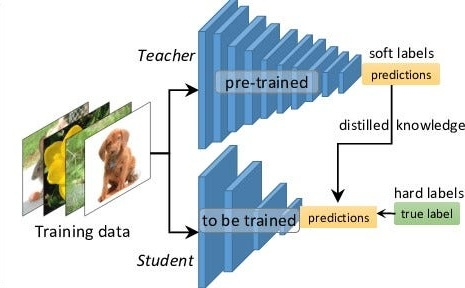
\includegraphics[width=0.7\linewidth]{figs/distillation.jpg}
    \caption{Distillation process. Source: \cite{kd_simplified}.}
    \label{fig:distillation}
\end{figure}

As shown in \autoref{fig:distillation}, the distillation typically trains the student the student model on a combination of the original dataset and the logits (soft outputs) produced by the teacher model. These outputs carry rich information about the data distribution, which aids the student model in capturing the nuances of complex decision boundaries. By leveraging the teacher model's expertise, the student model can learn more efficiently and produce results that are close to, and sometimes even surpass, the performance of the teacher model \cite{distilling}.

Kullback-Leibler (KL) Divergence loss \cite{kl} is a crucial aspect of the knowledge distillation training process. It quantifies the discrepancy between two probability distributions. Specifically, within the framework of model distillation, this loss assesses the divergence between the teacher and student model output distributions and allows you to train a student to minimize it.

The training loss is a linear combination (weighted sum) of the usual cross-entropy loss and KL divergence. The weight given to the distillation loss depends on the ratio of logits of the teacher and the student, making it adaptive and allowing the KL divergence component to have a more significant contribution when the teacher is more confident in the prediction than the student.

% As proposed by \citeauthor{multidistil} \cite{multidistil}, multiple teachers jointly train a single student in a unified framework. Various pre-trained teacher models are employed to generate soft labels for the training data. Consequently, each training data item comprises two elements: the golden label (the definitive binary label) determined by human judges and numerous soft labels (probabilistic labels ranging between 0 and 1) provided by the different teacher models. During the training, the student model, equipped with several headers, simultaneously learns from both the golden label and the soft labels. In the inference phase, the final decision is derived from a weighted combination of all outputs from the student headers. This concept is similar to the human learning process, where knowledge is acquired not from a single teacher but from multiple educators, leading to a more unbiased and comprehensive understanding.

Traditional model distillation is a crucial advancement in machine learning (ML). It enables the development of smaller, more efficient models that maintain the advanced understanding of their larger counterparts. However, these methods are not used extensively for the LLM\@.

\section{White-box LLM distillation}
\label{section:whitebox}

In the domain of white-box knowledge distillation for LLMs, the transparency of the teacher model's internal parameters is exploited to furnish student models with more detailed and practical training signals. This enhanced access can facilitate improved performance in the student models. One notable technique in white-box LLM distillation is the MiniLLM method, as documented in the \cite{minillm}.

KL divergence cannot be computed analytically in this context; instead it requires the the Monte Carlo method \cite{montecarlo} estimation. The inherent limitation of the student model, being less powerful, is that its probability distribution lacks the diversity found in the teacher model's distribution. Consequently, the student model's distribution tends to collapse onto a more straightforward geometric form, such as a line, which inadequately captures the complexities of the teacher model's distribution.

To address these discrepancies, \citeauthor{minillm} \cite{minillm} employ reverse KL divergence. This variant of KL divergence is particularly advantageous for knowledge distillation in generative language models, as it ``prevents the student model from overestimating the low-probability regions of the teacher distribution.'' Minimizing forward KL divergence causes the student model to place large probability masses on the zero-probability regions of the teacher model, corresponding to the generation of low-quality text in practice. To optimize this reverse KL divergence, authors use Policy Gradient \cite{policy_gradient}, adding complexity.

Authors of other white-box knowledge distillation for LLMs method SLIM \cite{slim} create a logits dataset (outputs of neurons without applying the activation function) through the teacher model from our training dataset. For each token in the sequence, we accordingly get $V$ (vocabulary size) values, which will be soft targets. The issue with this approach is that it demands significant space. To reduce the requirements, authors propose to take only the top $5\%$ of logits for each token, considering the rest as zeros, thus resulting in sparse logits.

\section{Black-box LLM distillation}

Beyond the white-box distillation, there is another concept of distillation when dealing with LLMs. This concept involves using the teacher model to generate prompts or tasks that can be incredibly informative for training the student model. This technique is called “prompt-based distillation.”

\citeauthor{socraticcot} \cite{socraticcot} introduce the approach called ``Socratic CoT\@.'' This method involves learning to split the initial problem into a series of small subproblems. These subproblems are then used to steer the intermediate steps of reasoning. To implement this, they train two compact prompt-distilled models: one for decomposing the problem and another for solving the subproblems.

Conversely, \citeauthor{stepbystep} \cite{stepbystep} propose a different method that also utilizes chain-of-thought (CoT) \cite{cot} prompting to extract rationales from an LLM\@. Then, authors utilize these rationales alongside the task labels to train student models. At its core, rationales offer a more in-depth insight into the reasoning behind associating an input with a particular output label. They frequently encapsulate pertinent task knowledge that might be challenging to deduce from the original inputs alone. Unlike the previous method, a student model trained in this way does not require pre-generated rationales to be applied to the test set.

The TinyLLM method \cite{tinyllm} improves the previous method by acquiring rationales from multiple LLMs. The authors introduce an optional in-context example generator to produce context-specific examples for a given input to ensure that these teacher-generated rationales are contextually grounded. The student model is trained through multi-task instruction tuning \cite{t5,t0}, including the ground truth label.

\section*{Conclusion}

While the literature on model distillation provides comprehensive insights into its application in ML, a noticeable research gap exists in the specific context of Large Language Models. The unique challenges posed by the immense size and complexity of LLM call for distillation techniques that currently need to be explored. Addressing this gap by developing or optimizing distillation methods specifically for LLM could significantly enhance their computational efficiency and broaden their practical applicability, especially in resource-limited scenarios. This area of research promises to advance the field of ML and make the benefits of LLM more accessible and sustainable.
